
\documentclass[12pt,letterpaper]{article}

\usepackage[margin=1in]{geometry}
\usepackage{amsmath,amssymb}
\usepackage{booktabs}
\usepackage{graphicx}
\usepackage{hyperref}
\usepackage{enumitem}
\usepackage{caption}
\usepackage{array}
\usepackage{parskip}
\usepackage{float}
\usepackage{tikz}
\usetikzlibrary{arrows.meta,calc}

\hypersetup{
    colorlinks=true,
    linkcolor=blue,
    urlcolor=blue
}


% ── tikz sketches for hydraulic jump classification ──────────────────────────
\newcommand{\jumpsketchsimple}{
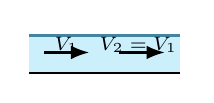
\begin{tikzpicture}[x=1cm,y=1cm,scale=0.48,>=Latex]
    \fill[cyan!20] (0,0.2) rectangle (4,1.2);
    \draw[thick,cyan!60!black] (0,1.2) -- (4,1.2);
    \draw[thick] (0,0.2) -- (4,0.2);
    \draw[->,thick] (0.4,0.75) -- (1.6,0.75);
    \draw[->,thick] (2.4,0.75) -- (3.6,0.75);
    \node[font=\scriptsize] at (1.0,0.95) {$V_1$};
    \node[font=\scriptsize] at (2.9,0.95) {$V_2=V_1$};
\end{tikzpicture}
}
\newcommand{\jumpsketchundulant}{
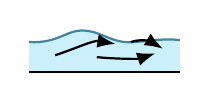
\begin{tikzpicture}[x=1cm,y=1cm,scale=0.48,>=Latex]
    \fill[cyan!20] (0,0.2) -- (0,1.0)
      .. controls (0.8,0.95) and (1.0,1.35) .. (1.5,1.30)
      .. controls (2.0,1.25) and (2.2,0.95) .. (2.8,1.00)
      .. controls (3.2,1.03) and (3.6,1.10) .. (4,1.05)
      -- (4,0.2) -- cycle;
    \draw[thick,cyan!60!black] (0,1.0)
      .. controls (0.8,0.95) and (1.0,1.35) .. (1.5,1.30)
      .. controls (2.0,1.25) and (2.2,0.95) .. (2.8,1.00)
      .. controls (3.2,1.03) and (3.6,1.10) .. (4,1.05);
    \draw[thick] (0,0.2) -- (4,0.2);
    \draw[->,thick] (0.7,0.65) .. controls (1.3,0.85) and (1.7,1.05) .. (2.3,0.95);
    \draw[->,thick] (1.8,0.6) .. controls (2.3,0.55) and (2.9,0.55) .. (3.35,0.7);
    \draw[->,thick] (2.7,1.0) .. controls (3.0,1.1) and (3.25,1.0) .. (3.55,0.82);
\end{tikzpicture}
}
\newcommand{\jumpsketchweak}{
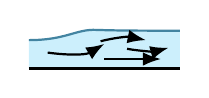
\begin{tikzpicture}[x=1cm,y=1cm,scale=0.48,>=Latex]
    \fill[cyan!20] (0,0.2) -- (0,0.95)
      .. controls (1.0,0.95) and (1.25,1.25) .. (1.8,1.22)
      .. controls (2.4,1.20) and (3.0,1.20) .. (4,1.20)
      -- (4,0.2) -- cycle;
    \draw[thick,cyan!60!black] (0,0.95)
      .. controls (1.0,0.95) and (1.25,1.25) .. (1.8,1.22)
      .. controls (2.4,1.20) and (3.0,1.20) .. (4,1.20);
    \draw[thick] (0,0.2) -- (4,0.2);
    \draw[->,thick] (0.5,0.62) .. controls (1.0,0.55) and (1.5,0.55) .. (2.0,0.85);
    \draw[->,thick] (1.9,0.92) .. controls (2.2,1.0) and (2.6,1.05) .. (3.1,0.95);
    \draw[->,thick] (2.0,0.45) -- (3.5,0.45);
    \draw[->,thick] (2.6,0.72) .. controls (3.0,0.65) and (3.35,0.65) .. (3.7,0.75);
\end{tikzpicture}
}
\newcommand{\jumpsketchoscillating}{
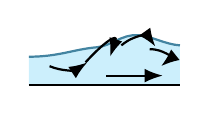
\begin{tikzpicture}[x=1cm,y=1cm,scale=0.48,>=Latex]
    \fill[cyan!20] (0,0.2) -- (0,0.95)
      .. controls (0.8,0.95) and (1.2,1.15) .. (1.8,1.20)
      .. controls (2.2,1.24) and (2.45,1.55) .. (2.9,1.52)
      .. controls (3.3,1.48) and (3.6,1.28) .. (4,1.25)
      -- (4,0.2) -- cycle;
    \draw[thick,cyan!60!black] (0,0.95)
      .. controls (0.8,0.95) and (1.2,1.15) .. (1.8,1.20)
      .. controls (2.2,1.24) and (2.45,1.55) .. (2.9,1.52)
      .. controls (3.3,1.48) and (3.6,1.28) .. (4,1.25);
    \draw[thick] (0,0.2) -- (4,0.2);
    \draw[->,thick] (0.55,0.7) .. controls (0.9,0.55) and (1.25,0.6) .. (1.55,0.8);
    \draw[->,thick] (1.5,0.8) .. controls (2.05,1.4) and (2.35,1.55) .. (2.15,0.95);
    \draw[->,thick] (2.45,1.25) .. controls (2.8,1.55) and (3.15,1.5) .. (3.35,1.22);
    \draw[->,thick] (2.05,0.45) -- (3.55,0.45);
    \draw[->,thick] (3.2,1.15) .. controls (3.6,1.15) and (3.75,0.9) .. (3.5,0.7);
\end{tikzpicture}
}
\newcommand{\jumpsketchstable}{
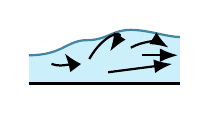
\begin{tikzpicture}[x=1cm,y=1cm,scale=0.48,>=Latex]
    \fill[cyan!20] (0,0.2) -- (0,0.95)
      .. controls (0.9,0.95) and (1.0,1.35) .. (1.55,1.35)
      .. controls (2.1,1.35) and (2.2,1.65) .. (2.8,1.62)
      .. controls (3.3,1.58) and (3.6,1.45) .. (4,1.43)
      -- (4,0.2) -- cycle;
    \draw[thick,cyan!60!black] (0,0.95)
      .. controls (0.9,0.95) and (1.0,1.35) .. (1.55,1.35)
      .. controls (2.1,1.35) and (2.2,1.65) .. (2.8,1.62)
      .. controls (3.3,1.58) and (3.6,1.45) .. (4,1.43);
    \draw[thick] (0,0.2) -- (4,0.2);
    \draw[->,thick] (0.6,0.72) .. controls (0.95,0.6) and (1.1,0.8) .. (0.95,1.0);
    \draw[->,thick] (1.6,0.85) .. controls (2.0,1.55) and (2.5,1.6) .. (2.15,1.05);
    \draw[->,thick] (2.7,1.15) .. controls (3.05,1.35) and (3.45,1.3) .. (3.7,1.15);
    \draw[->,thick] (2.1,0.5) -- (3.8,0.72);
    \draw[->,thick] (3.0,0.95) -- (3.95,0.95);
\end{tikzpicture}
}
\newcommand{\jumpsketchrough}{
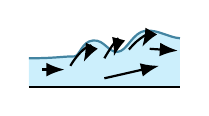
\begin{tikzpicture}[x=1cm,y=1cm,scale=0.48,>=Latex]
    \fill[cyan!20] (0,0.2) -- (0,0.95)
      .. controls (0.7,0.95) and (0.9,1.0) .. (1.2,1.0)
      .. controls (1.35,1.0) and (1.4,1.4) .. (1.7,1.42)
      .. controls (2.0,1.45) and (2.1,1.1) .. (2.35,1.12)
      .. controls (2.6,1.13) and (2.75,1.65) .. (3.1,1.68)
      .. controls (3.45,1.7) and (3.7,1.5) .. (4,1.48)
      -- (4,0.2) -- cycle;
    \draw[thick,cyan!60!black] (0,0.95)
      .. controls (0.7,0.95) and (0.9,1.0) .. (1.2,1.0)
      .. controls (1.35,1.0) and (1.4,1.4) .. (1.7,1.42)
      .. controls (2.0,1.45) and (2.1,1.1) .. (2.35,1.12)
      .. controls (2.6,1.13) and (2.75,1.65) .. (3.1,1.68)
      .. controls (3.45,1.7) and (3.7,1.5) .. (4,1.48);
    \draw[thick] (0,0.2) -- (4,0.2);
    \draw[->,thick] (0.35,0.65) -- (0.95,0.65);
    \draw[->,thick] (1.1,0.75) .. controls (1.4,1.25) and (1.7,1.35) .. (1.45,0.85);
    \draw[->,thick] (2.0,0.95) .. controls (2.2,1.3) and (2.4,1.55) .. (2.25,1.0);
    \draw[->,thick] (2.65,1.18) .. controls (2.95,1.55) and (3.2,1.6) .. (3.0,1.25);
    \draw[->,thick] (2.0,0.42) -- (3.45,0.75);
    \draw[->,thick] (3.2,1.2) -- (3.95,1.15);
\end{tikzpicture}
}

\begin{document}

% ── title page ────────────────────────────────────────────────────────────────
\begin{titlepage}
\centering
\vspace*{1.5cm}

{\Large MIE312: Lab 1\par}
\vspace{0.5em}
{\Huge\bfseries Open Channel Flow\par}
\vspace{1.5em}

{\Large Department of Mechanical and Industrial Engineering\par}
{\Large University of Toronto\par}
\textcolor{white}{\Large Prepared by: Prof. Sullivan} \\
{\Large Fall 2026}
\vfill

\begin{figure}[htbp]
    \centering
    % trim = <left> <bottom> <right> <top>
    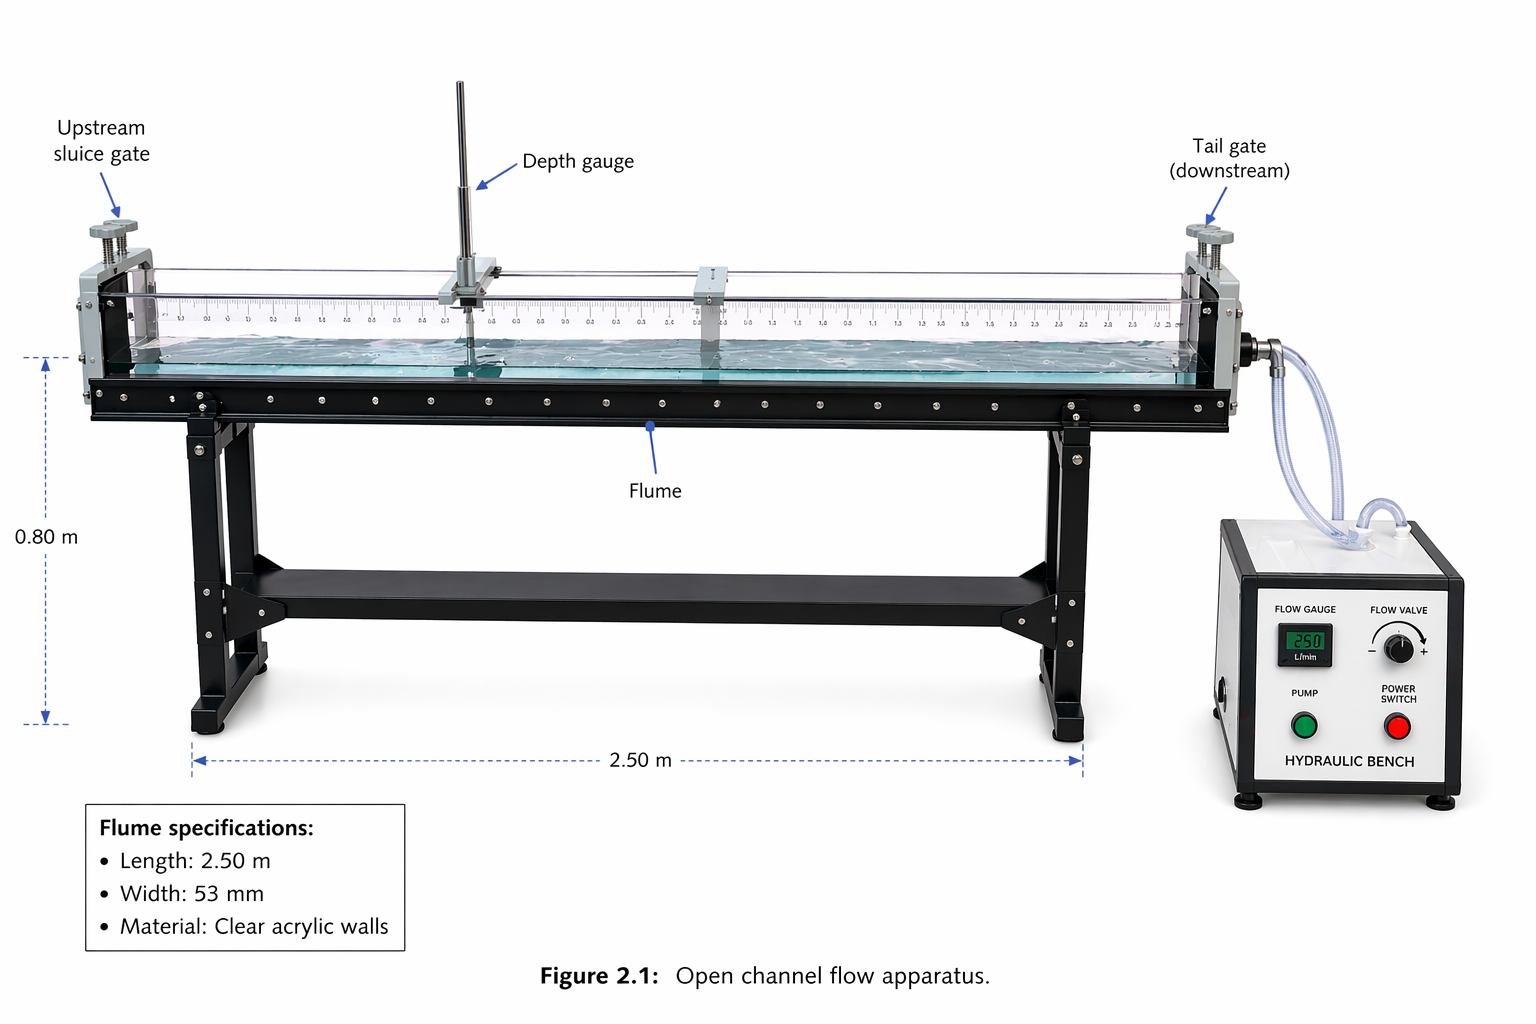
\includegraphics[trim=0 60pt 0 0, clip, width=0.85\textwidth]{Figures/cover_apparatus.png}
    \caption{Open channel flow apparatus.}
    \label{fig:apparatus_cover}
\end{figure}

\vfill

\begin{tabular}{|p{0.32\textwidth}|p{0.38\textwidth}|}
\hline
Teaching Assistant: & Muhan Yu \\ \hline
Email: & \texttt{muhan.yu@mail.utoronto.ca} \\ \hline
\end{tabular}

\vfill
\end{titlepage}

% ── companion notebook ────────────────────────────────────────────────────────
\section*{Companion Notebook}

A  Google Colab notebook accompanies this lab manual. It automates the calculations, generates report-ready plots, and provides a concise summary once raw measurements are entered.

\begin{center}
\href{https://colab.research.google.com/github/pierresullivan/mie312-labs/blob/main/lab1-flume/MIE312_Lab1_Open_Channel_Flow.ipynb}{\textbf{Open the MIE312 Lab 1 Colab Notebook}}
\end{center}

\subsection*{How to use the notebook}
\begin{enumerate}[leftmargin=*, label=\arabic*.]
    \item Open the notebook link and select \textbf{File $\to$ Save a copy in Drive}.
    \item Run the setup cells to define constants and helper functions.
    \item Enter your measured values in the data-entry tables for Bernoulli verification, sill flow, and hydraulic jump.
    \item Run the remaining cells to compute theoretical values, Froude number, and head-loss quantities automatically.
    \item Copy the generated tables, plots, and summary text into your report as needed.
\end{enumerate}
\vspace{1em}
\hrule
\vspace{1em}

\section{Objective}
The objectives of this lab experiment are to:
\begin{itemize}[leftmargin=*]
    \item verify the Bernoulli equation,
    \item study the effect of a submerged object on the channel flow,
    \item generate and recognize hydraulic jump.
\end{itemize}

\section{Experimental Setup}
Figure~\ref{fig:apparatus} shows a schematic of the apparatus used in this experiment.

\begin{itemize}[leftmargin=*]
    \item \textbf{Flume:} A long open channel with clear walls that can be used to store or allow the flow of water. The flume used in this laboratory is \(2.5\,\text{m}\) long and \(53\,\text{mm}\) wide.
    \item \textbf{Sluice gate:} Located at the head of the flume and can be installed fully opened, partially opened, or fully closed. It should be installed with the sharper edge facing upstream. It controls the depth of the water flowing into the flume on one side and maintains the head of the water on the other side.
    \item \textbf{Tail gate:} Similar to the sluice gate except that it is located at the end of the flume. It can be raised up or down to control the depth of the downstream water at the tail of the flume.
    \item \textbf{Sill:} A smooth and flat object placed on the floor of the flume to analyze water flow over it. It has the shape of an equilateral trapezoid.
    \item \textbf{Hydraulic Bench:} Pumping unit consisting of the Power Switch, Pump, Flow Valve, and digital Flow Gauge. The pump drives the water from the internal water tank to the flume. The flow rate from the hydraulic bench to the flume is controlled by the Flow Valve.
\end{itemize}

It is essential to let the flow stabilize for about \(5\) minutes after each step in the experiment to obtain accurate results.

\begin{figure}[H]
    \centering
    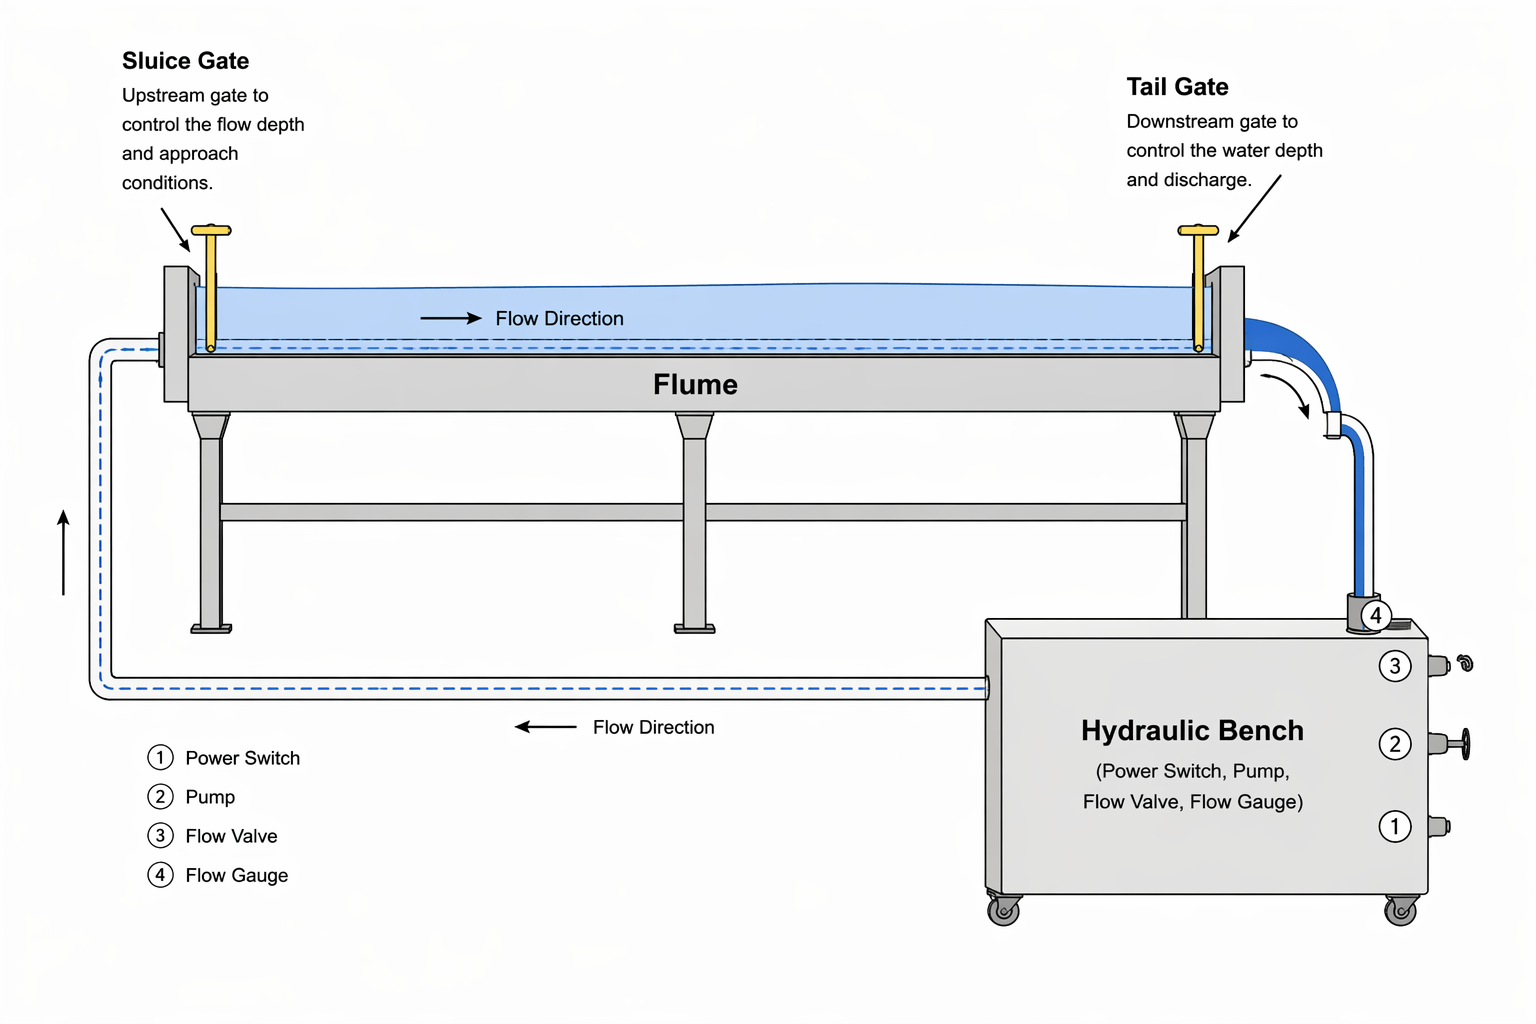
\includegraphics[width=0.9\textwidth]{Figures/apparatus.png}
    \caption{Open Channel Flow Apparatus}
    \label{fig:apparatus}
\end{figure}

\section{Theoretical Background}

\subsection{The Bernoulli Equation}
The Bernoulli equation is fundamentally an energy conservation equation along a streamline in the fluid flow. If friction is negligible, any two points along a streamline have the same energy:
\begin{equation}
p_1 + \frac{1}{2}\rho V_1^2 + \gamma z_1
=
p_2 + \frac{1}{2}\rho V_2^2 + \gamma z_2
\label{eq:bernoulli-general}
\end{equation}
where \(p\) is pressure, \(\rho\) is density, \(V\) is velocity, \(\gamma\) is specific weight, and \(z\) is elevation. When Bernoulli's equation is applied between points on the \emph{free surface}, both points are exposed to atmosphere and therefore \(p_1=p_2=0\) gauge pressure. At submerged locations, however, the pressure is hydrostatic and should not be set to zero.

\subsubsection*{Derivation used in Part 5.1}
For the sluice-gate configuration, let section \(1\) be the upstream region of depth \(H\), and section \(2\) be the flow under the gate of depth \(h\). The flume width is constant, so continuity gives
\begin{equation}
Q = bHV_1 = bhV_2
\quad\Longrightarrow\quad
V_1 = \frac{h}{H}V_2.
\label{eq:continuity-sluice}
\end{equation}
For a horizontal rectangular open channel with hydrostatic pressure distributions and kinetic-energy correction factors taken as approximately unity, the section-averaged energy equation is
\begin{equation}
H + \frac{V_1^2}{2g}
=
h + \frac{V_2^2}{2g}.
\label{eq:bernoulli-sluice}
\end{equation}
This form already includes the hydrostatic pressure contribution across each section. It is therefore important \emph{not} to set the pressure at the section centroid to atmospheric pressure; only the free surface is at atmospheric pressure.

Substituting \(V_1=(h/H)V_2\) into Eq.~\eqref{eq:bernoulli-sluice},
\begin{align}
H + \frac{1}{2g}\left(\frac{h}{H}\right)^2 V_2^2
&=
h + \frac{V_2^2}{2g}, \\
\frac{V_2^2}{2g}\left[1-\left(\frac{h}{H}\right)^2\right]
&=
H-h.
\end{align}
Hence
\begin{equation}
V_2^2
=
\frac{2g(H-h)}{1-(h/H)^2}
=
\frac{2g(H-h)}{(H^2-h^2)/H^2}
=
\frac{2gH^2}{H+h}.
\end{equation}
Therefore,
\begin{equation}
\boxed{V_2 = \sqrt{\frac{2gH^2}{H+h}}}.
\label{eq:sluice-velocity-derived}
\end{equation}
When \(h\ll H\), this approaches the familiar reservoir estimate \(V_2\approx\sqrt{2gH}\).

\subsection{Hydraulic Jump}
A hydraulic jump is characterized by the sudden change in the depth of the water layer over a short distance. It always increases the depth of the water layer in the direction of the flow. The upstream shallower flow has a higher velocity than the downstream deeper flow, so part of the kinetic energy is dissipated in turbulence.

\begin{figure}[H]
    \centering
    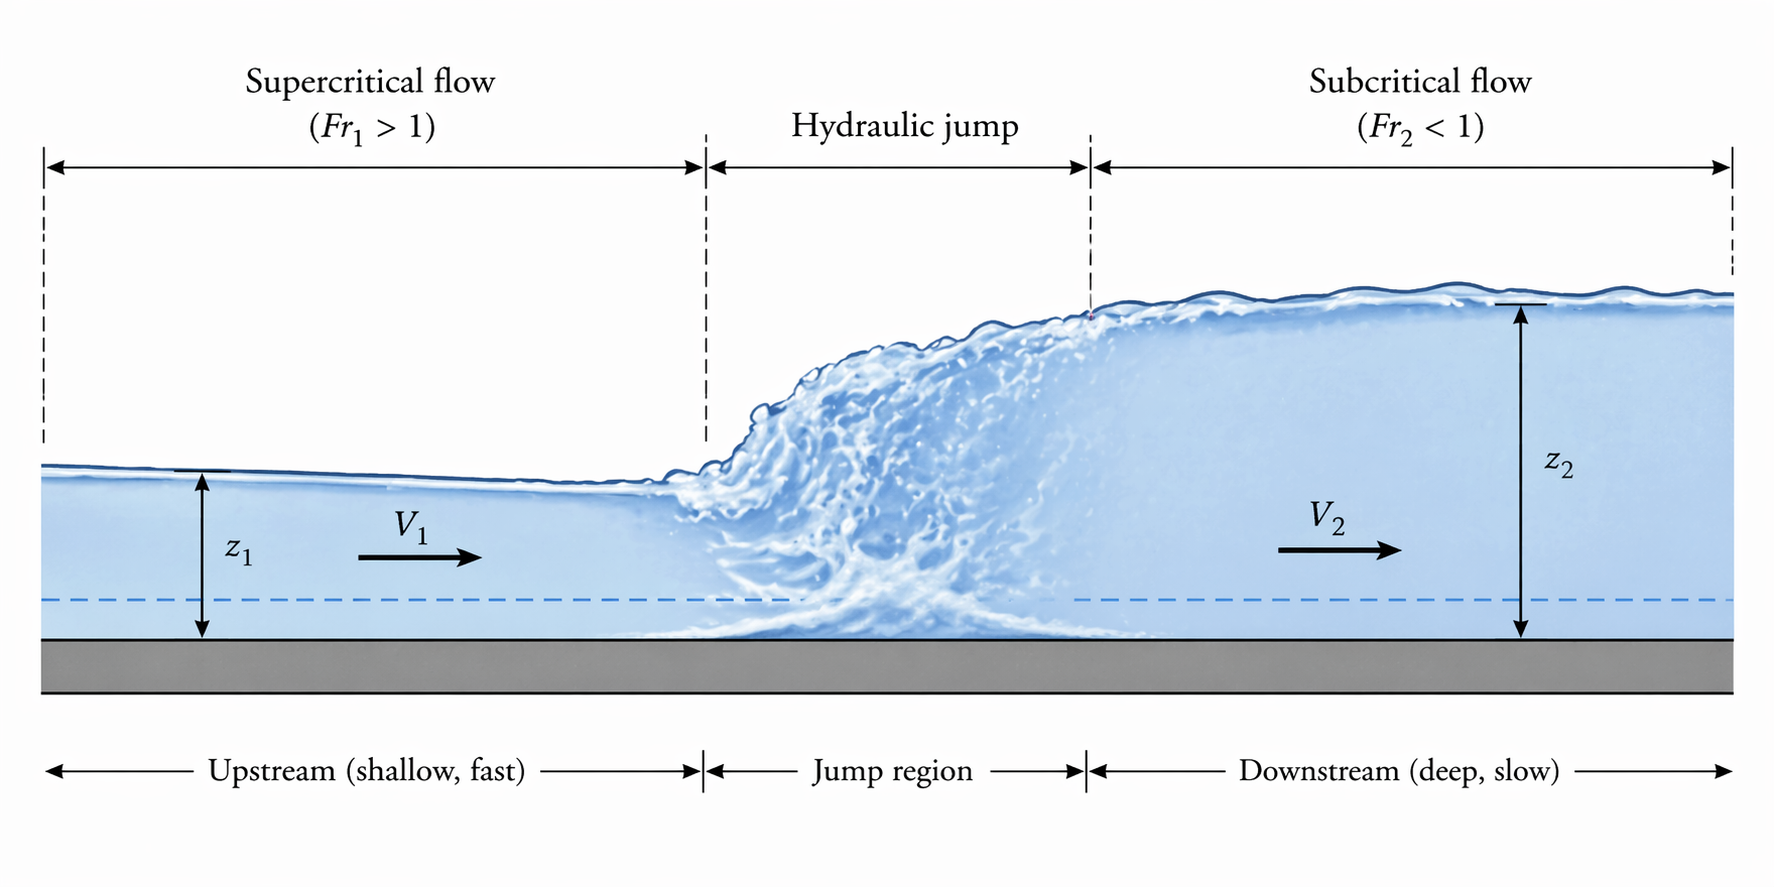
\includegraphics[width=0.9\textwidth]{Figures/hyd_jump_nature.png}
    \caption{Hydraulic jump showing the upstream velocity \(V_1\) and downstream velocity \(V_2\).}
    \label{fig:hydraulic-jump-natural}
\end{figure}

A very important, but not sufficient, condition for hydraulic jump is that the flow before the jump must be supercritical. The Froude number is
\begin{equation}
Fr = \frac{V}{\sqrt{gz}}
\label{eq:froude}
\end{equation}
where \(z\) is the local flow depth. Supercritical flow corresponds to \(Fr>1\), subcritical flow corresponds to \(Fr<1\), and \(Fr=1\) is the critical limiting condition. A hydraulic jump requires a supercritical upstream state, so in practice \(Fr_1>1\).

Applying continuity and the linear-momentum equation to a control volume spanning the jump leads to the conjugate-depth relation
\begin{equation}
\frac{z_2}{z_1}
=
\frac{1}{2}\left(-1+\sqrt{1+8Fr_1^2}\right).
\label{eq:jump-depth-ratio}
\end{equation}


\begin{table}[H]
\centering
\caption{Different types of hydraulic jumps}
\label{tab:jumpclass}
\renewcommand{\arraystretch}{1.45}
\setlength{\tabcolsep}{6pt}
\begin{tabular}{|m{0.11\textwidth}|m{0.11\textwidth}|m{0.43\textwidth}|m{0.24\textwidth}|}
\hline
\centering \textbf{\(Fr_1\)} &
\centering \textbf{\(z_2/z_1\)} &
\centering \textbf{Classification} &
\centering \textbf{Sketch}
\tabularnewline
\hline
\centering \(<1\) &
\centering \(1\) &
Jump impossible &
\centering \jumpsketchsimple
\tabularnewline
\hline
\centering \(1<Fr_1\le 1.7\) &
\centering \(1\) to \(2.0\) &
Standing wave or undulant jump &
\centering \jumpsketchundulant
\tabularnewline
\hline
\centering \(1.7\) to \(2.5\) &
\centering \(2.0\) to \(3.1\) &
Weak jump &
\centering \jumpsketchweak
\tabularnewline
\hline
\centering \(2.5\) to \(4.5\) &
\centering \(3.1\) to \(5.9\) &
Oscillating jump &
\centering \jumpsketchoscillating
\tabularnewline
\hline
\centering \(4.5\) to \(9.0\) &
\centering \(5.9\) to \(12\) &
Stable, well-balanced steady jump; insensitive to downstream conditions &
\centering \jumpsketchstable
\tabularnewline
\hline
\centering \(>9.0\) &
\centering \(>12\) &
Rough, somewhat intermittent strong jump &
\centering \jumpsketchrough
\tabularnewline
\hline
\end{tabular}
\label{tab:jump-types}
\end{table}


\section{Procedure}
Use the depth gauge for all depth measurements. First use the depth gauge to measure the distance to the flume floor, \(f\), then to the water height, \(w\). The water depth is \(d=w-f\).

\subsection{Verify the Bernoulli Equation}
\begin{enumerate}[leftmargin=*]
    \item Raise the tail gate fully and remove the sluice gate if installed.
    \item Start the water pump by pressing the black power button mounted on the system. Use the flow control valve to set the flow to \(25\,\text{L/min}\). At any time, the system can be shut down by pressing the red button.
    \item Wait until the water starts flowing through the flume.
    \item Install and lower the upstream sluice gate such that \(H\) is around \(55\,\text{mm}\) and \(h\) is roughly \(8\,\text{mm}\) (Figure~\ref{fig:sluice}).
\begin{figure}
    \centering
    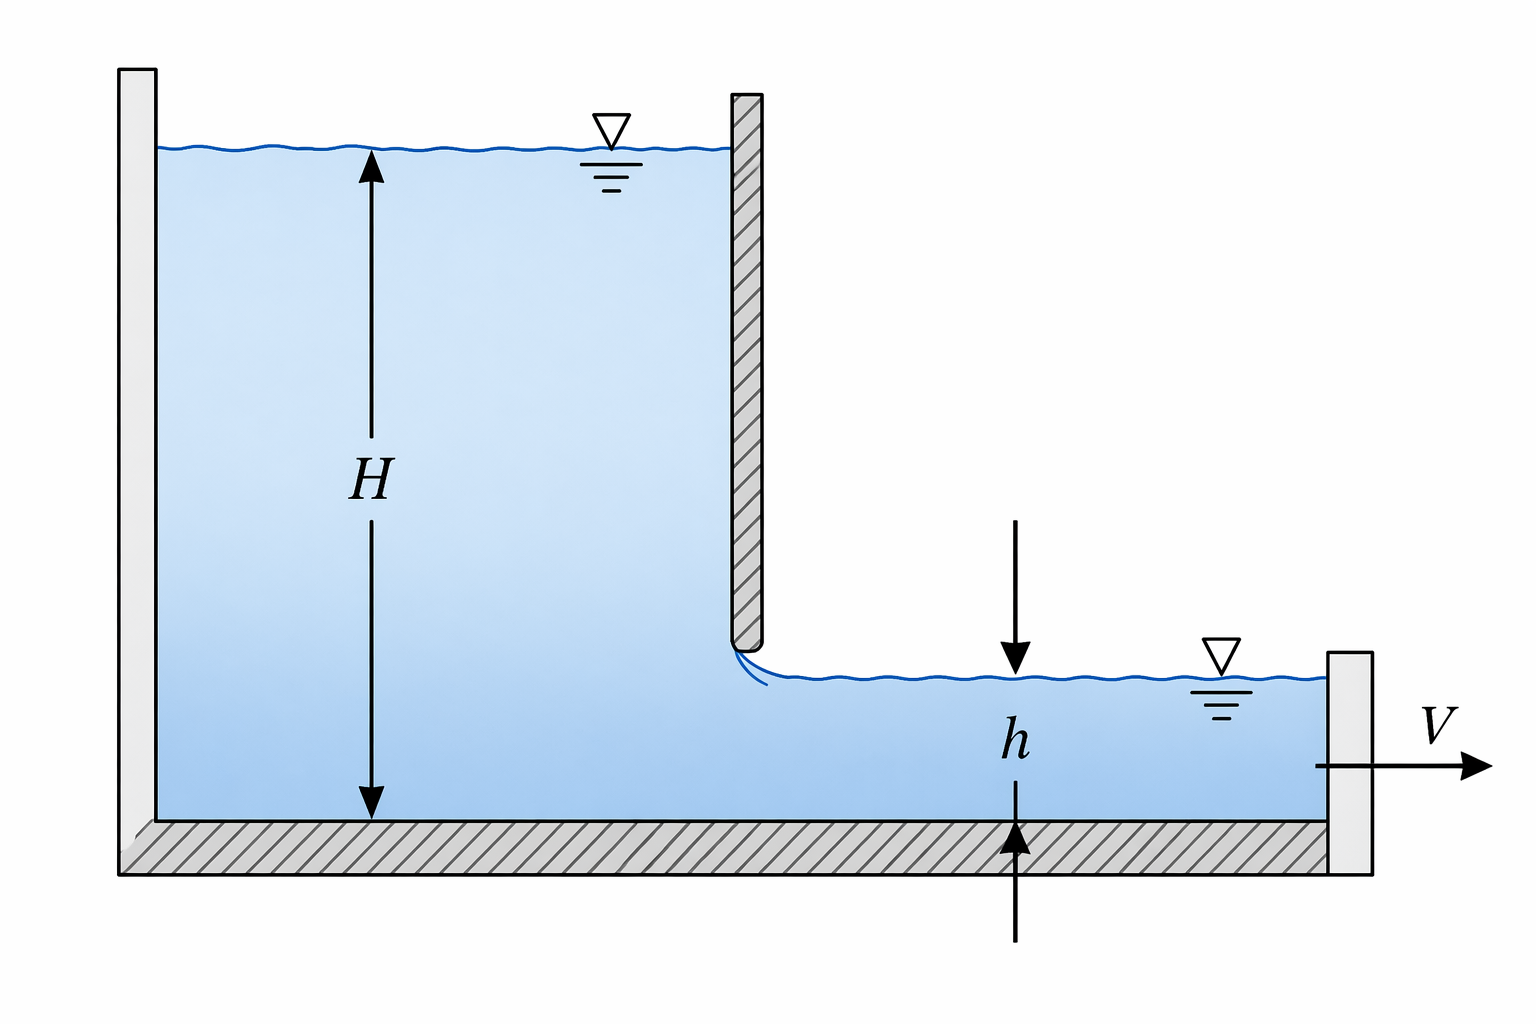
\includegraphics[width=0.8\linewidth]{Figures/sluice_gate.png}
    \caption{Flow under the sluice gate}
    \label{fig:sluice}
\end{figure}
    \item Measure \(V\) about halfway downstream by dividing the overall flow rate by the flow area \(\bigl(Q/(53\,\text{mm}\times h)\bigr)\).
    \item Repeat steps 4 and 5 again with different values of \(H\) and \(h\), and record them in Table~\ref{tab:bernoulli}.
    \item Turn off the water pump.
    \item Remove the sluice gate and raise the end gate to maximum height.
\end{enumerate}

\begin{table}[H]
\centering
\caption{Velocity measurement downstream of sluice gate}
\label{tab:bernoulli}
\small
\begin{tabular}{cccc>{\centering\arraybackslash}p{0.28\textwidth}}
\toprule
Trial No. & \(H\) (mm) & \(h\) (mm) & Flow Rate, \(Q\) (L/min) & Calculated velocity downstream (m/s) \\
\midrule
1 & & & & \\
2 & & & & \\
\bottomrule
\end{tabular}
\end{table}

\subsection{Flow over a Submerged Sill}
\begin{enumerate}[leftmargin=*]
    \item Raise the tail gate fully and remove the sluice gate if installed.
    \item Place the sill into the flume around the \(1400\,\text{mm}\) mark. Ensure the sill sits properly on the floor of the flume and does not float in water.
    \item Turn the water pump on and set to \(45\,\text{L/min}\). Record the flow rate \(Q\) in Table~\ref{tab:sill}.
    \item Adjust the tail gate such that the upstream depth of the flow is \(60\,\text{mm}\).
    \item The free surface of the flow will dip as it passes over the sill. If it does not, lower the tail gate to generate the dip.
    \item Measure \(y_1\), \(y_2\), and \(\Delta\) as defined in Figure~\ref{fig:sill} and record them in Table~\ref{tab:sill}.
\end{enumerate}

\begin{figure}[H]
    \centering
    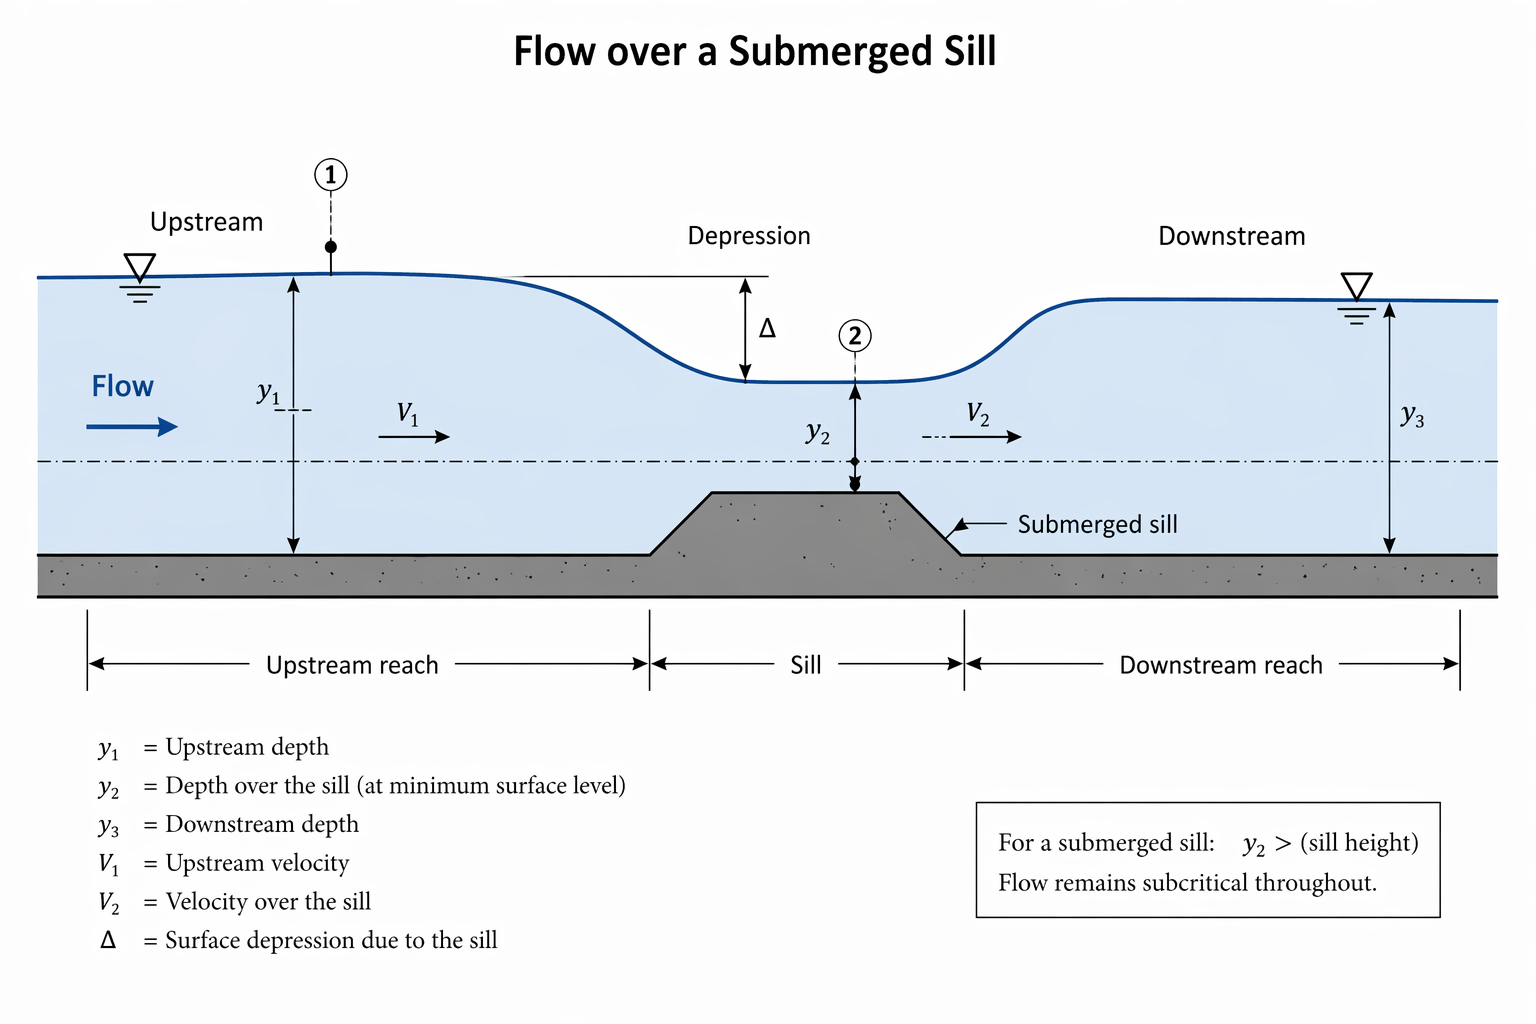
\includegraphics[width=0.82\textwidth]{Figures/sill_flow.png}
    \caption{Flow over a submerged sill and the surface dip \(\Delta\)}
    \label{fig:sill}
\end{figure}

\begin{table}[H]
\centering
\caption{Measurements for the flow over a submerged sill}
\label{tab:sill}
\begin{tabular}{cccc}
\toprule
\(Q\) (L/min) & \(y_1\) (mm) & \(y_2\) (mm) & \(\Delta\) (mm) \\
\midrule
 & & & \\
\bottomrule
\end{tabular}
\end{table}

\subsection{Hydraulic Jump}
\begin{enumerate}[leftmargin=*]
    \item Raise the tail gate fully and remove the sluice gate if installed.
    \item Start the water pump and use the flow control valve to set the flow to \(25\,\text{L/min}\).
    \item Wait until the water starts flowing through the flume.
    \item Install and lower the upstream sluice gate such that \(H\) is around \(75\,\text{mm}\) and \(h\) is roughly \(10\,\text{mm}\). Record the value in Table~\ref{tab:jump}.
    \item Attempt to create a hydraulic jump by lowering and adjusting the tail gate.
    \item Measure the height \(z_1\) before the hydraulic jump and the height \(z_2\) after the hydraulic jump.
    \item Find velocities \(V_1\) and \(V_2\) using \(z_1\), \(z_2\), and the dimensions of the flume.
    \item Shut down the apparatus; open the end gate fully, close the main flow valve, and turn off the pump.
\end{enumerate}

\begin{table}[H]
\centering
\caption{Measurements for the hydraulic jump}
\label{tab:jump}
\begin{tabular}{ccccc}
\toprule
\(H\) (mm) & \(z_1\) (mm) & \(z_2\) (mm) & \(V_1\) (m/s) & \(V_2\) (m/s) \\
\midrule
 & & & & \\
\bottomrule
\end{tabular}
\end{table}

\section{Questions for Analysis}

\subsection{Verify the Bernoulli Equation}
\begin{enumerate}[leftmargin=*]
    \item Use Bernoulli’s equation to predict the velocity \(V\) assuming the depths \(H\) and \(h\) are known; specifically, show the derived expression used for the flow under the sluice gate.
    \item Using the equation in the previous question and the height values recorded in Table~\ref{tab:bernoulli}, find the theoretical velocity.
    \item Compare the theoretical velocity values with the measured velocity values. What can you conclude about the validity of Bernoulli’s equation? If these values differ, briefly comment on the sources of error.
\end{enumerate}

\subsection{Flow over a Submerged Sill}
\subsubsection*{Derivation used in Part 5.2}
Consider section \(1\) upstream of the sill and section \(2\) at the dip location over the sill. Since both sections are open to atmosphere, \(p_1=p_2=0\). Applying Bernoulli along the free surface gives
\begin{equation}
z_{s,1} + y_1 + \frac{V_1^2}{2g}
=
z_{s,2} + y_2 + \frac{V_2^2}{2g},
\end{equation}
where \(z_{s,1}\) and \(z_{s,2}\) are the bed elevations. By the geometry of the surface dip,
\begin{equation}
\Delta = (z_{s,1}+y_1) - (z_{s,2}+y_2)
= \frac{V_2^2 - V_1^2}{2g}.
\label{eq:delta-bernoulli}
\end{equation}
Continuity in a rectangular channel of constant width gives
\begin{equation}
Q = by_1V_1 = by_2V_2
\quad\Longrightarrow\quad
V_2 = V_1\frac{y_1}{y_2}.
\label{eq:sill-continuity}
\end{equation}
Substituting Eq.~\eqref{eq:sill-continuity} into Eq.~\eqref{eq:delta-bernoulli},
\begin{align}
\Delta
&=
\frac{1}{2g}\left[V_1^2\left(\frac{y_1}{y_2}\right)^2 - V_1^2\right] \\
&=
\frac{V_1^2}{2g}\left[\left(\frac{y_1}{y_2}\right)^2 - 1\right].
\label{eq:sill-dip-derived}
\end{align}

\begin{enumerate}[leftmargin=*]
    \item Using Bernoulli’s equation, show that the dip \(\Delta\), as defined in Figure~\ref{fig:sill}, is
    \[
    \Delta =
    \frac{V_1^2}{2g}
    \left[
    \left(\frac{y_1}{y_2}\right)^2 - 1
    \right].
    \]
    \item Find the velocity \(V_1\) using the flow rate \(Q\):
    \begin{equation}
    V_1 = \frac{Q}{b\,y_1},
    \qquad b = 53\,\text{mm}.
    \end{equation}
    \item Find the theoretical value of the dip using the equation above and compare it to the measured value in Table~\ref{tab:sill}. Does Bernoulli’s equation also hold true for the flow with a submerged sill? If these values differ, comment on any sources of error that may have affected your results.
\end{enumerate}

\subsection{Hydraulic Jump}
\begin{enumerate}[leftmargin=*]
    \item Describe the region at the onset of hydraulic jump.
    \item Find the Froude number, \(Fr_1\), of the flow before the hydraulic jump using Eq.~\eqref{eq:froude}. What kind of flow is it (supercritical or subcritical)?
    \item Using the theoretical equation
    \[
    \frac{z_2}{z_1}
    =
    \frac{1}{2}\left(-1+\sqrt{1+8Fr_1^2}\right),
    \]
    find the value of \(Fr_1\) and compare it to the value of \(Fr_1\) found in the previous question.
    \item Based on the \(z_2/z_1\) value and Table~\ref{tab:jumpclass}, classify the hydraulic jump.
    \item The head loss \(h_L\) due to the hydraulic jump is given by
    \[
    \frac{h_L}{z_1}
    =
    1-\frac{z_2}{z_1}
    +
    \frac{Fr_1^2}{2}
    \left[
    1-\left(\frac{z_1}{z_2}\right)^2
    \right].
    \]
    Find \(h_L\). Also find the ratio of \(h_L\) to the overall maximum energy of the flow. Is \(h_L\) significant compared to the overall maximum energy? Use Bernoulli’s equation to support your discussion.
\end{enumerate}

\section{Recommended Text Readings}

To fully prepare for the experimental and computational components of these labs, students are strongly encouraged to review the relevant sections in the course textbook. The following readings provide the theoretical foundation for the phenomena observed in the laboratory.

\vspace{0.3cm}
\noindent\textbf{Course Textbook Reference:} \\
White, F. M., \& Xue, H. (2020). \textit{Fluid Mechanics} (9th ed.). McGraw-Hill Education. \\
\textit{(*Note: Chapter and section numbering remains consistent with the 8th edition.)}
\vspace{0.3cm}

\subsection*{Lab 1: Bernoulli Equation and Open Channel Flow}
\textbf{Primary Focus:} Energy conservation, ideal flow, and free-surface phenomena (sluice gates, sills, and hydraulic jumps).
\begin{itemize}
    \item \textbf{Chapter 3: Integral Relations for a Control Volume}
    \begin{itemize}
        \item Section 3.5: The Bernoulli Equation (Derivation and restrictions)
        \item Section 3.7: The Energy Equation (Kinetic energy correction factor, $\alpha$)
    \end{itemize}
    \item \textbf{Chapter 10: Open-Channel Flow} 
    
    \begin{itemize}
        \item Section 10.1: Introduction to Froude Number and Wave Speed
        \item Section 10.4: The Hydraulic Jump
        \item Section 10.5: Flow over a Submerged Sill/Weir
    \end{itemize}

    \item \textbf{Supplementary References:}
    \begin{itemize}
        \item Henderson, F. M. (1966). \textit{Open Channel Flow}. Macmillan. \textit{(The classical authoritative text on hydraulic jumps and channel transitions).}
        \item National Committee for Fluid Mechanics Films (NCFMF). \textit{Waves in Fluids}. \textit{(Excellent visual demonstrations of free-surface flow phenomena).} \url{https://www.youtube.com/watch?v=MNyebpog_i0&list=PL0EC6527BE871ABA3&index=19}
    \end{itemize}
\end{itemize}





\end{document}
